\documentclass{article}


% Packages
\usepackage[utf8]{inputenc} % For Norwegian letters
\usepackage{tabulary} % For nice tables
\usepackage{enumerate}
\usepackage{float}
\usepackage{graphicx}

% Config
\setlength{\parindent}{0cm}
\setlength{\parskip}{\baselineskip}%

\begin{document}

% Title
\title{\textbf{Exercise 1} \\ 4173}
\author{Simon Borøy-Johnsen \\ MTDT}
\date{\today}
\maketitle
% End Title


% Content

% Task 1
\section{Theory}

\subsection{Basic Concepts}

\subsubsection{}
A well-posed learning problem is expressed in three terms; task \textit{T}, performance \textit{P}, and experience \textit{E}. A program is able to learn if it can improve its performance \textit{P} at task \textit{T} given its experience \textit{E}.

\begin{tabulary}{\textwidth}{|L|L|L|L|}
    \hline
    \textbf{Problem} & \textbf{Task} & \textbf{Performance} & \textbf{Experience} \\\hline
    Play tic-tac-toe & Winning tic-tac-to games & Percent of games won & Opportunity to play against oneself \\\hline
    Automatic face recognition & Correctly recognize faces in photos & Percentage of faces correctly recognized & Set of photos with manually recognized faces \\\hline
\end{tabulary}

\subsubsection{}
Inductive bias is a set of assertions that the learning algorithm uses to classify outputs given inputs it has not encountered before.

In machine learning, we use training data in order to solve general problems. Without the bias, the algorithm won't recognize problems it hasn't encountered before, and the algorithm will only be able to solve training data problems. The inductive bias is important for machine learning because it allows us to solve problems never encountered before.

Candidate elimination uses representation bias. It assumes that the underlying concept is a part of the hypothesis space.

ID3 uses preference bias. It arranges decision nodes in order of their projected information gain. It follows the principle of Occam's razor; preferring the shortest hypothesis that fits the data.

\subsubsection{}
Overfitting occurs when the algorithm is too well fitted to the training data. The model is then too complex to accurately match other data than in the training examples.

We say that a hypothesis \textit{h} overfits the training data if there exists and alternative hypothesis \textit{h'}, such that $error_{training}(h)<error_{training}(h')$ and $error_{data}(h)>error_{data}(h')$.

\subsection{Concept Learning}

\subsubsection{}

\subsubsection*{Training}
Initial \\
$G=\{\langle ?, ?, ?, ?, ? \rangle\}$ \\
$S=\{\langle \emptyset, \emptyset, \emptyset, \emptyset, \emptyset \rangle\}$

Example 1 \\
$G=\{\langle ?, ?, ?, ?, ? \rangle\}$ \\
$S=\{ Hair, Live, False, False, Flat \}$

Example 2 \\
$G=\{\langle Hair, ?, ?, ?, ? \rangle, \langle ?, Live, ?, ?, ? \rangle, \langle ?, ?, False, ?, ? \rangle, \langle ?, ?, ?, False, ? \rangle, \langle ?, ?, ?, ?, Flat \rangle\}$ \\
$S=\{ Hair, Live, False, False, Flat \}$

Example 3 \\
$G=\{\langle Hair, ?, ?, ?, ? \rangle, \langle ?, Live, ?, ?, ? \rangle, \langle ?, ?, False, ?, ? \rangle, \langle ?, ?, ?, False, ? \rangle\}$ \\
$S=\{ Hair, Live, False, False, ? \}$

\subsubsection*{Classification}
Example 1 \\
$\langle Hair, Live, False, False, None \rangle \rightarrow True$

Example 2 \\
$\langle Leathers, Egg, False, True, Pointed \rangle \rightarrow Unknown$

Example 3 \\
$\langle Scales, Egg, True, False, Flat \rangle \rightarrow Unknown$

\subsubsection{}
The first classification example matches both the general and the special boundaries, and is therefore classified as a mammal. The two other examples does not match, and we can therefore say nothing about their classification.

\subsubsection{}
The system should ask for an example that gains as much useful information about the classification examples as possible.

$\langle Scales, Egg, True, False, Pointed \rangle \rightarrow False$

% Task 2
\section{Programming}

\begin{enumerate}
    \item See main.py.
    \item 
        \begin{enumerate}[a)]
            \item The initial values of W and b are all randomized uniformly in the range [-1.0, 1.0]. This was done in order to avoid the algorithm being stuck with "worst case" training values. $\alpha$ is set to 0.5. This value was found using trial and error. The value is constant due to the simple complexity of the problem space.
            \item Iteration 5: 0.028577 (MSE). \\
                  Iteration 10: 0.020971 (MSE).
            \item Final results: 0.002544 (MSE). For change of loss function, see Figure [\ref{fig:plot}].
        \end{enumerate}
\end{enumerate}


\begin{figure}[H]
  \centering
  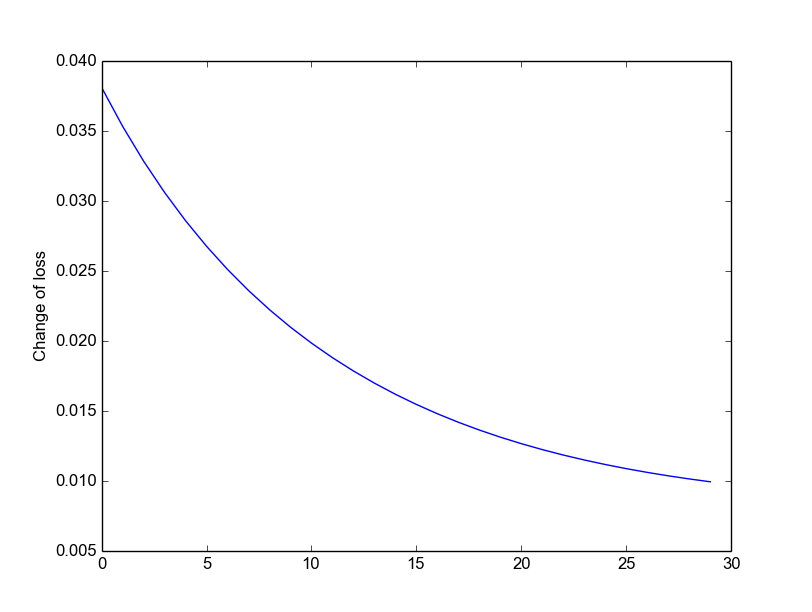
\includegraphics[width=1.0\textwidth]{figures/plot.png}
  \caption{Plot of the loss function for each iteration until the target error (0.01) was reached.}
  \label{fig:plot}
\end{figure}

% End content

\end{document}
